\documentclass[a4paper, 12pt]{article}%тип документа

%отступы
\usepackage[left=2cm,right=2cm,top=2cm,bottom=3cm,bindingoffset=0cm]{geometry}

%Русский язык
\usepackage[T2A]{fontenc} %кодировка
\usepackage[utf8]{inputenc} %кодировка исходного кода
\usepackage[english,russian]{babel} %локализация и переносы

%Вставка картинок
\usepackage{graphicx}
\graphicspath{{pictures/}}
\DeclareGraphicsExtensions{.pdf,.png,.jpg}

%Графики
\usepackage{pgfplots}
\pgfplotsset{compat=1.9}

%Математика
\usepackage{amsmath, amsfonts, amssymb, amsthm, mathtools}

%Заголовок
\author{Валеев Рауф Раушанович \\
группа 825}
\title{Работа 1.3.2 \\
Определение модуля кручения}
\begin{document}
\maketitle
\newpage
\textbf{Цель работы:} измерение углов закручивания в зависимости от приложенного момента сил, расчет модулей кручения и сдвига при статическом закручивании стержня, определение тех же модулей для проволоки по измерениям периодов крутильных колебаний подвешенного на ней маятника (динамическим методом).

\textbf{В работе используется:} в первой части: исследуемый стержень, отсчетная труба со шкалой, рулетка, микрометр, набор грузов; во второй части: проволока из иследуемого материала, грузы, секундомер, микрометр, рулетка, линейка.

\center{\textbf{Определение модуля кручения стержня статистическим методом}}

\begin{figure}[h]
\center{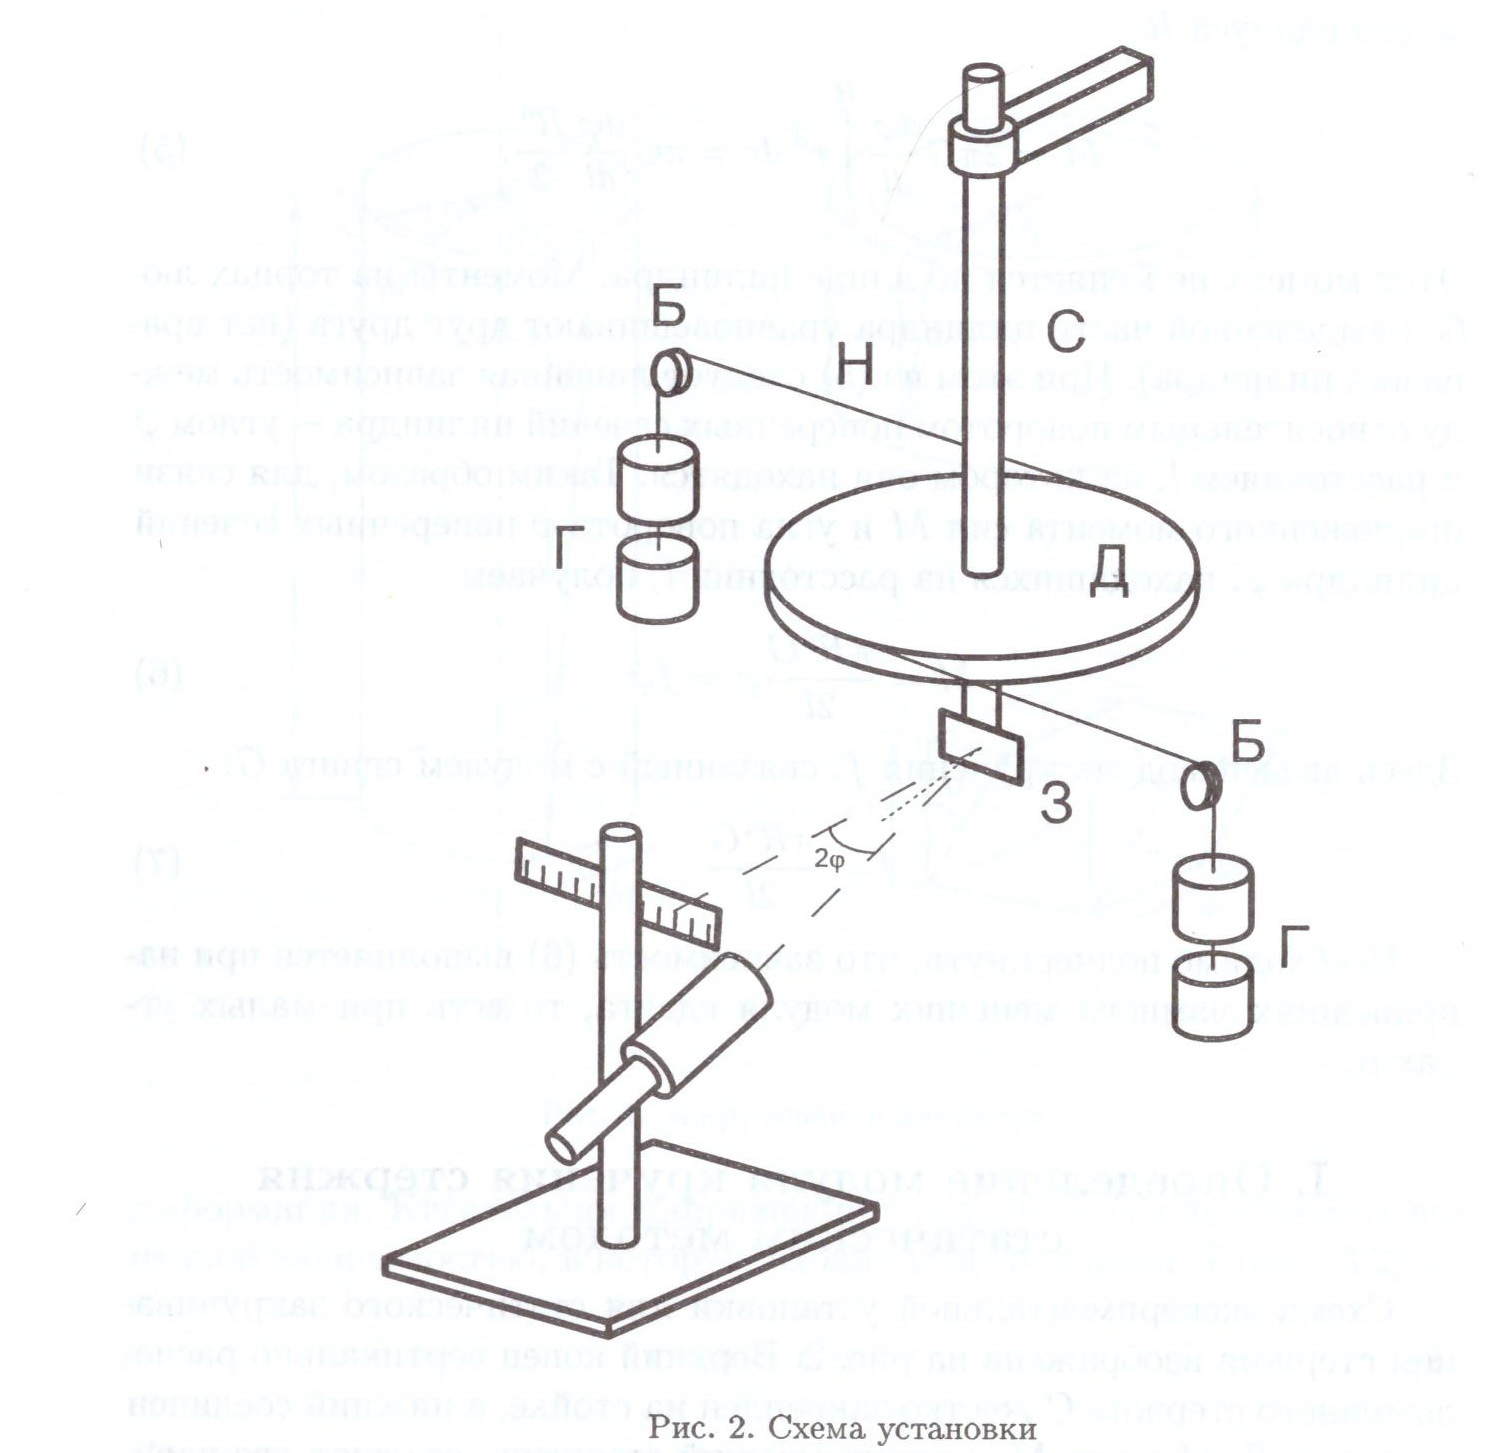
\includegraphics{132_1.jpg}}
\end{figure}
\begin{enumerate}
\item Измеряем R цилиндра (табл.1).
\item Устанавливаем зрительную трубку таким образом, чтобы в нее четко было видно отражение шкалы в зеркальце З. Измеряем расстояние от зеркальца З до шкалы. Определяем диаметр стержня С и шкива Д.
\item Увеличивая нагрузку на нитях Н, снимаем зависимость аналогично 2 части 1.3.1 $\phi = \phi (M)$. Проделаем эксперимент в обратном порядке, постепенно уменьшая велечину закручивающего момента. Повторяем измерения не менее трех раз (табл. 1). 
\item Результаты эксперимента изображаем графически в координатах ($\phi$, М). При помощи этих графиков определяем велечину модуля кручения f. 
\item Используя формулу 
\[G = \dfrac{2lf}{\pi R^4}\]
, где $ M = mgr$, где $r = 5,23\pm0,01 cm$ - радиус нижнего диска;
Вычисляем модуль сдвига. Сравниваем полученное значение с табличным. 
\end{enumerate}
%\newpage
\begin{table}
\center{
\begin{tabular}{|c|c|c|c|c|c|c|c|c|}
\hline
phi&0,022&0,051&0,084&0,104&0,104&0,085&0,055&0,031\\
\hline
M,Н*м&0,1047&0,210&0,314&0,409&0,409&0,314&0,210&0,105\\
\hline
\hline
phi&0,022&0,054&0,087&0,110&0,110&0,087&0,060&0,030\\
\hline
M,Н*м&0,1047&0,210&0,314&0,409&0,409&0,314&0,210&0,105\\
\hline
\hline
phi&0,021&0,049&0,079&0,103&0,103&0,084&0,060&0,025\\
\hline
M,Н*м&0,1047&0,210&0,314&0,409&0,409&0,314&0,210&0,105\\
\hline
\end{tabular}
}
\caption{Зависимость угла от массы}
\begin{tabular}{|c|c|c|c|}
\hline
&Значение&$\sigma$&$\varepsilon$\\
\hline
f кг/рад&3,68&0,47&0,13\\
\hline
G $*10^{10}$ $\text{Н}/\text{м}^2$ &9,31&0,34&0,04\\
\hline
\end{tabular}
\caption{Значения}
\end{table}
\begin{tikzpicture}
\begin{axis} [title = Зависимость удлинения проволоки от нагрузки,
		xlabel=$\Delta l \text{, мм}$,
		ylabel= {M, Н*м}]
\addplot coordinates {
(0.104, 0.022)
(0.104, 0.021)
(0.104, 0.031)
(0.104, 0.030)
(0.104, 0.025)
(0.104, 0.022)
(0.210, 0.051)
(0.210, 0.054)
(0.210, 0.049)
(0.210, 0.055)
(0.210, 0.06)
(0.210, 0.06)
(0.314, 0.084)
(0.314, 0.087)
(0.314, 0.079)
(0.314, 0.085)
(0.314, 0.087)
(0.314, 0.084)
(0.409, 0.104)
(0.409, 0.110)
(0.409, 0.103)
};
\addplot coordinates {
(0, 0.000)
(0.5, 0.133)
};
\end{axis}
\end{tikzpicture}
\end{document}